% -*-coding: utf-8 -*-

\documentclass[compress,mathserif]{beamer}

\usepackage[utf8]{inputenc}
\usepackage[czech]{babel}
\usepackage[IL2]{fontenc}
\usepackage{amsmath}
\usepackage{amsthm}
\usepackage{amssymb}
\usepackage{amstext}
\usepackage{graphicx}
\usepackage{booktabs}
\usepackage{multirow}
\usepackage{dcolumn}

\newcolumntype{d}{D{,}{,}{4.2}}
\newcolumntype{k}{D{,}{,}{2}}
\newcolumntype{j}{D{,}{,}{1}}
\newcolumntype{u}{D{,}{,}{0}}

% Definice makra pro české uvozovky:
\def\bq{\mbox{\kern.1ex\protect\raisebox{-1.3ex}[0pt][0pt]{''}\kern-.1ex}}
\def\eq{\mbox{\kern-.1ex``\kern.1ex}}
\def\ifundefined#1{\expandafter\ifx\csname#1\endcsname\relax }%
\ifundefined{uv}%
        \gdef\uv#1{\bq #1\eq}
\fi

% beamer setup
\usetheme{Warsaw}
\beamertemplateballitem

\theoremstyle{definition}
\newtheorem{define}{Definice}

\theoremstyle{plain}
\newtheorem{thm}{Věta}

\newcommand{\beI}{\begin{itemize}}
\newcommand{\enI}{\end{itemize}}
\newcommand{\bL}{\mathbf{L}}


\title{Paralelní implementace fuzzy filtrů ve zpracování obrazu na GPU}
\author{Ladislav Horký}
\institute{FJFI ČVUT v Praze \newline \newline Vedoucí práce: Ing. Tomáš Oberhuber Ph.D.
\newline Konzultant: doc. Ing. Jaromír Kukal Ph.D.}
\date{\today} 

\begin{document}
% úvodní slidy
	\begin{frame}
		\titlepage
	\end{frame}
	
	\section*{Obsah}   % nebude v obsahu
	\begin{frame}{Obsah}
		\tableofcontents
	\end{frame}

\section{Výsledky}
    \begin{frame}{Testovací sestava}
        \begin{table}
        \begin{tabular}{lcc}
          \toprule
          & CPU & GPU \\
          \midrule
          \multirow{2}{*}{Název} & Intel & NVIDIA \\
          & Core 2 DUO & GeForce 8800 GTX \\
          Výpočetní & 2 & 128 \\
          jednotky & (využita 1) & (4 SM $\times$ 32 CUDA-jader) \\
          Frekvence & 1860 MHz & 1400 MHz \\
          Výpočetní & \multirow{2}{*}{---} & \multirow{2}{*}{1.0} \\
          schopnost & & \\ 
          Cache & 2 MB L2 & --- \\
          RAM/DRAM & 2 GB DDR2 & 768 MB GDDR3 \\
          FSB & 800 MHz & 1800 MHz \\
          \bottomrule
        \end{tabular}
        %\caption{Testovací sestava}
        \end{table}
    \end{frame}
    
    \begin{frame}{Urychlení morfologických filtrů}
        \begin{table}
        %\hspace{-0.1cm}
        \begin{tabular}{lkuku}
          \toprule
          Maska $\rightarrow$ & \multicolumn{2}{c}{kapacita masky: 26} & \multicolumn{2}{c}{kapacita masky: 18}\\
          Filtr $\downarrow$ & \multicolumn{1}{c}{GPU (ms)} & \multicolumn{1}{c}{Urychlení} & \multicolumn{1}{c}{GPU (ms)} & \multicolumn{1}{c}{Urychlení}\\
          \midrule
          \multicolumn{5}{c}{{\tt unsigned char} (0-255)}  \vspace{0.1cm} \\
          Eroze     & 1,47 & \textbf{30,2} & 1,34 & \textbf{24,0}\\
          Dilatace  & 1,47 & \textbf{30,3} & 1,37 & \textbf{23,8}\\
          Hrany     & 1,56 & \textbf{51,8} & 1,35 & \textbf{43,2}\\
          \midrule
          \multicolumn{5}{c}{{\tt unsigned int} (0-65535)}  \vspace{0.1cm} \\
          Eroze     & 1,61 & \textbf{31,0} & 1,37 & \textbf{26,9}\\
          Dilatace  & 1,62 & \textbf{30,9} & 1,37 & \textbf{27,1}\\
          Hrany     & 1,53 & \textbf{51,4} & 1,32 & \textbf{43,5}\\
          \bottomrule
        \end{tabular}
        %\caption{Srovnání morfologických filtrů na CPU a GPU pro různé datové typy}
        \end{table}
    \end{frame}

     \begin{frame}{Urychlení morfologických filtrů}
        \begin{table}
        %\hspace{-0.1cm}
        \begin{tabular}{lkuku}
          \toprule
          Maska $\rightarrow$ & \multicolumn{2}{c}{kapacita masky: 26} & \multicolumn{2}{c}{kapacita masky: 18}\\
          Filtr $\downarrow$ & \multicolumn{1}{c}{GPU (ms)} & \multicolumn{1}{c}{Urychlení} & \multicolumn{1}{c}{GPU (ms)} & \multicolumn{1}{c}{Urychlení}\\
          \midrule
           \multicolumn{5}{c}{{\tt unsigned char} (0-255)}  \vspace{0.1cm} \\
          Medián        & 9,45     & \textbf{33,9} & 3,62   & \textbf{58,3}\\
          BES           & 10,17    & \textbf{37,1} & 4,98   & \textbf{53,1}\\
          H-L Medián    & 735,76   & \textbf{4,3}  & 342,34 & \textbf{4,9} \\
          WBES          & 1124,46  & \textbf{4,2}  & 463,81 & \textbf{5,4} \\
          \midrule
          \multicolumn{5}{c}{{\tt unsigned int} (0-65535)}  \vspace{0.1cm} \\
          Medián        & 25,24    & \textbf{12,4} & 5,96   & \textbf{34,6} \\
          BES           & 10,95    & \textbf{35,6} & 6,45   & \textbf{42,5} \\
          H-L Medián    & 1327,99  & \textbf{2,3}  & 434,21 & \textbf{3,8}  \\
          WBES          & 1328,10  & \textbf{3,6}  & 520,38 & \textbf{4,9}  \\
          \bottomrule
        \end{tabular}
        %\caption{Srovnání morfologických filtrů na CPU a GPU pro různé datové typy}
        \end{table}
    \end{frame}
    
    \begin{frame}{Ukázky}
    
    \begin{columns}
    \begin{column}{0.3\textwidth}
        \begin{table}
          \begin{tabular}{ll}
            Originál \hfill & Hrany \hfill\\
            \vspace{2.5cm} & \\
            Eroze  & Dilatace \\
          \end{tabular}
        \end{table}
    \end{column} 
    
    \begin{column}{0.6\textwidth}  
    \begin{figure}
     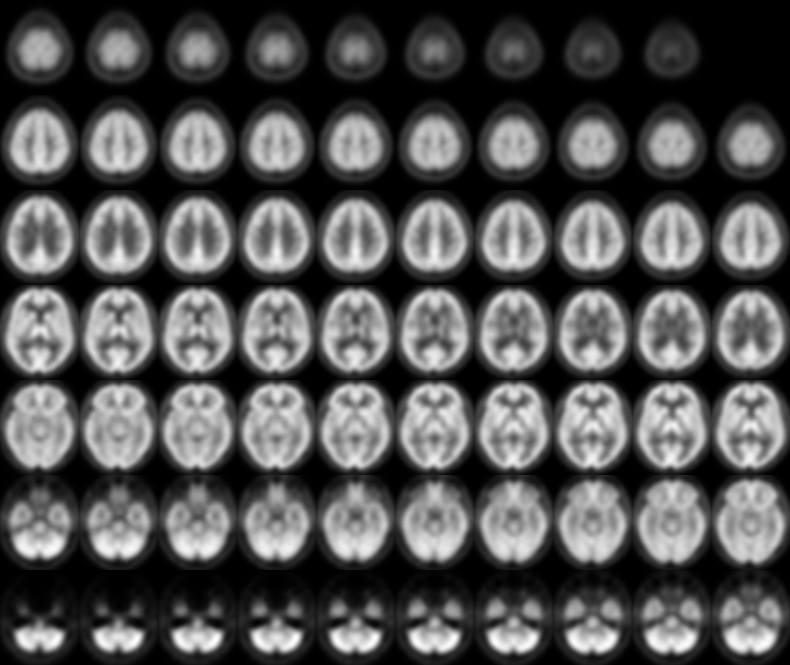
\includegraphics[width = 70pt]{img/original.png}
             \hspace{10pt}
     
\includegraphics[width = 70pt]{img/hrany.png}
    \end{figure}
    \vspace{-10pt}
    \begin{figure}
    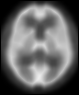
\includegraphics[width = 70pt]{img/eroze.png}
         \hspace{10pt}
    
\includegraphics[width = 70pt]{img/dilatace.png}
    \end{figure}
    \end{column}
    \end{columns}
        
    
    \end{frame}

\section{Závěr}
    \begin{frame}{Závěr}
      
    \end{frame}

\end{document}